\chapter{Implementation}\label{ch:implementation}
I det kommende afsnit, er løsningen blevet implementeret. Nu med planlægningen af kode (Analyse og design) er det muligt, at gå igang med næste aktivtitet under Unified Procces, implementation\cite{UnifiedProcess}. 

Koden er skrevet ud fra designklassediagrammet \ref{fig:designclassdiagram}, og benytter sig af de designmønstre som er vist i designklassediagrammet. Koden er skrevet i Java. 
De vigtigste metoder og designmønstre vil blive demonstreret, herunder parallelitet, singleton mønstret, database queries, og relevante algoritmer.

\todo{insert code snips, especially the stuff relevant to the database, our architecture, parallelity, and of course our regression algorithm.}


En måde at beregne den optimale bestillingsmængde af en given vare, ud fra hvornår det betaler sig bedst, er ved at bruge en formel, bedre kendt som Economic Order Quantity (EOQ) Model \cite{EOQ}. Denne formel beregner bestillingsmængden ud fra efterspørgsel, pris per hjembestilling, kostpris per enhed og gennemsnitlig inventaromkostninger. Denne formel tager dog ikke højde for parametre såsom årstid, temperatur på dagen, antal solgt per dag, osv. For at kunne finde den optimale bestillingsmængde løbende, med et ønske om at altid have nok af alle varer på lager, kan parametre måned, temperatur, og daglige salg, bruges med regression. Regression er en teknik, hvorved man kan bestemme det statistiske forhold mellem to eller flere variabler, hvor ændringer i en dependent-variabel er associeret med, og afhænger af, én eller flere uafhængige variabler. Det bliver i dette projekt brugt til at forudsige f.eks. hvor mange Isbåde\cite{Isbåd} der skal bestilles over de næste uger, eller perioder. Når bestillingsmængden over tid når op til EOQ bestillingsmængden ville bestillingen af varen foretages.

%Shouldn't put in a figure of a formula we aren't using.
%\begin{landscape}
%    \begin{figure}[p]
%        \centering
%        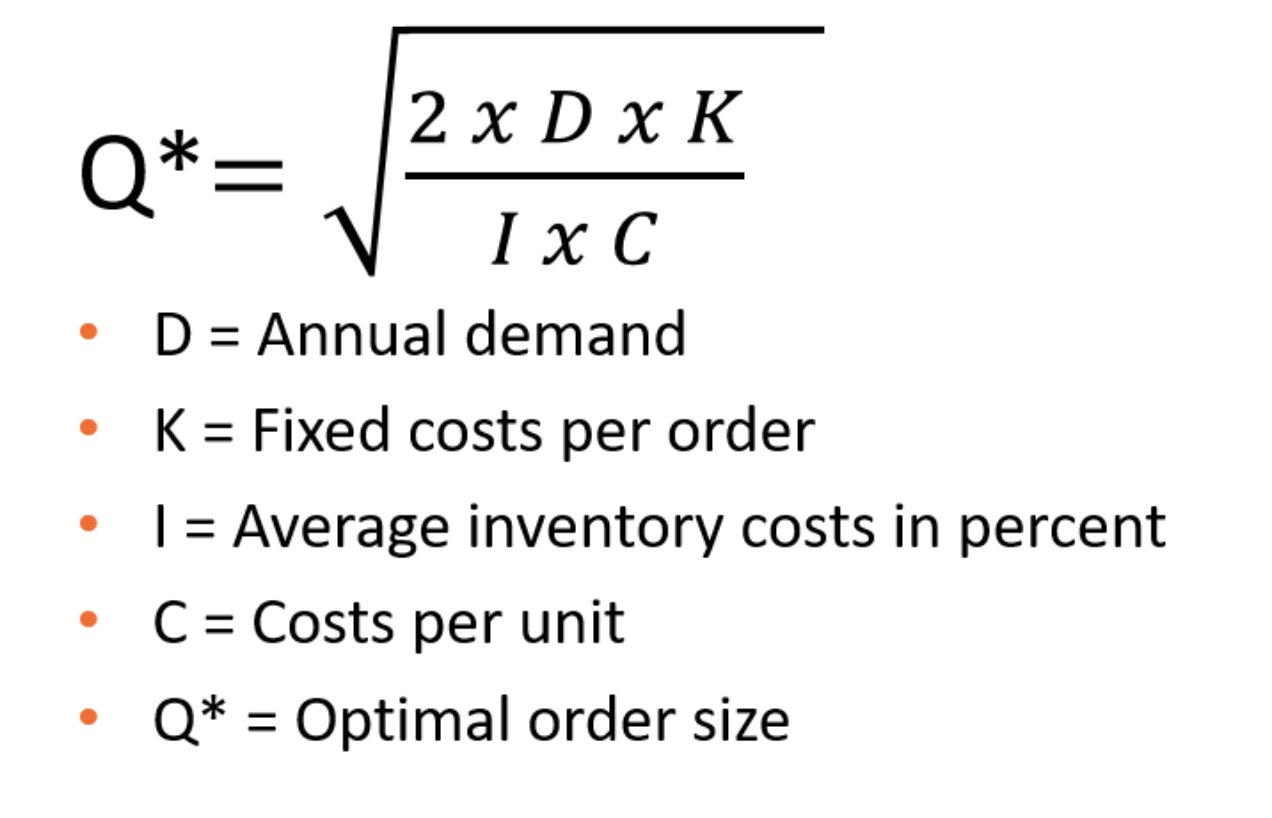
\includegraphics[width=\hsize]{figures/implementation/eoq.png}
%        \caption{EOQ formlen - Beregning af den optimale bestillingsmængde}
%        \label{fig:eoq}
%    \end{figure}
%\end{landscape}

Der kan så laves en \verb|productMap|, som lægges i \verb|PeriodicPlan| så der kan oprettes \verb|StorageOrder|s med de optimale bestillingsmængder. Desværre blev denne feature ikke implementeret færdig.

\section{Parallelitet}\label{ch:parallelitet}
Parallelitet er processen hvorved at dele af et program, kan køres på samme tid. Dele af programmer, som køres parallelt kaldes \texttt{Threads}\cite{JavaThreads}. Threads af en abstraktion, som benyttes i high-level programmerings sprog, som f.eks Java\cite{HighLevel}. Threads er meget ofte ydeevne-optimerende, eftersom at en moderne CPU meget ofte har flere kerner, hvilket resultere i at koden fra en thread ikke er afhængig af eksekveringen af koden fra en anden thread. Dette scenarie er det dog kun relevant, hvis der eksekveres en svær algoritme. Threads er også ydeevne-optimerende når det kommer til IO, eftersom at IO operationer ofte er langsommere, ift. læsning fra RAM eller læsning fra CPU cache\cite{OperatingSystems}. Et scenerie hvor et program henter mange forskellige billeder fra internettet~\ref{lst:badParralelExample}, er i dette eksempel \texttt{fetchImage(n)} som ses på kodeeksempel \ref{lst:badParralelExample}. Den henter billedet med ID fra en remote server, hvilket ikke er optimalt, fordi metoden \texttt{fetchAllTheImages} først venter på det første kald af \texttt{fetchImage} før den starter det næste. I dette eksempel har resultatet af første \texttt{fetchImage} kald ingen effekt på det næste. Det vil sige at metoden kunne blive paralleliseret~\ref{lst:goodParralelExample} og alle \texttt{fetchImage} metoder, som bruger ~100\% af eksekveringenstiden på at vente på et IO svar, kan køre på samtidigt. I denne nye version har vi stadig det samme loop, der er dog nogle ændringer: \texttt{finalI} er lavet fordi \texttt{i} kan ændre sig før Thread'en bliver kaldt. Dette resulterer i \texttt{fetchImage} metoder, der henter de forkerte billeder. I stedet for at kalde \texttt{fetchImage} metoden, så laves en Thread, som kalder den. 
Dernest lægges den i \texttt{threads} listen, og til sidst kaldes \texttt{join} metoden på alle threads for at sikre de er færdige før \texttt{fetchAllTheImages} afsluttes.

\begin{listing}
    \begin{minted}
    [
        frame=lines,
        framesep=2mm,
        baselinestretch=1.2,
        bgcolor=LightGray,
        fontsize=\footnotesize,
        linenos
    ]{java}
public void fetchAllTheImages(int index) {
    for(int i = 0; i < index; i++) {
        fetchImage(i + 1);
    }
}
    \end{minted}
    \caption{Eksempel på ingen brug af parallelitet\label{lst:badParralelExample}}
\end{listing}

\begin{listing}
    \begin{minted}
    [
        frame=lines,
        framesep=2mm,
        baselinestretch=1.2,
        bgcolor=LightGray,
        fontsize=\footnotesize,
        linenos
    ]{java}
public void fetchAllTheImages(int index) {
    List<Thread> threads = new ArrayList<>();
    for(int i = 0; i < index; i++) {
        final int finalI = i + 1;
        Thread thread = new Thread(() -> fetchImage(finalI));
        thread.start();
        threads.add(threads);
    }
    for(Thread thread : threads){
        try {
            thread.join();
        } catch (InterruptedException ignored) {

        }
    }
}
    \end{minted}
    \caption{Eksempel på ingen brug af parallelitet\label{lst:goodParralelExample}}
\end{listing}

Et godt brug at parallelitet i dette projekt kan findes i metoden \texttt{save()} i klassen \texttt{PeriodicPlanController}~\ref{lst:ourParralelExample}, her er alle 3 \texttt{store.update()} samt \texttt{store.delete()} langsomme IO operationer, så denne metode gør som~\ref{lst:goodParralelExample}, laver parallelitet med threads, starter dem, og til sidsts venter på de er færdige.     
 
\begin{listing}
    \begin{minted}
    [
        frame=lines,
        framesep=2mm,
        baselinestretch=1.2,
        bgcolor=LightGray,
        fontsize=\footnotesize,
        linenos
    ]{java}
    public void save() {
        Thread deleteThread = new Thread(() -> {
            try {
                store.delete(toDelete);
            } catch (DataAccessException ignored) {

            }
        });
        Thread update1Thread = new Thread(() -> {
            try {
                store.update(left, false);
            } catch (DataAccessException ignored) {

            }
        });
        Thread update2Thread = new Thread(() -> {
            try {
                store.update(current);
            } catch (DataAccessException ignored) {

            }
        });
        Thread update3Thread = new Thread(() -> {
            try {
                store.update(right, false);
            } catch (DataAccessException ignored) {

            }
        });
        deleteThread.start();
        update1Thread.start();
        update2Thread.start();
        update3Thread.start();
        try {
            deleteThread.join();
            update1Thread.join();
            update2Thread.join();
            update3Thread.join();
        } catch (InterruptedException ignored) {

        }
    }}
    \end{minted}
    \caption{Eksempel på ingen brug af parallelitet\label{lst:ourParralelExample}}
\end{listing}

\section{UI}
%Skriv lidt om UI
%Vi prioriterede funktionalitet meget i 1. iteration
%Brugte skrifttype valgt fra \ref{skrifttype}
%UI er "barebones" fordi funktionalitet > brugervenlighed i starten
%Kan det den skal ud fra Diagrammer
